\subsection{\textsf{PN}: A \DSL for (Simple) Petri Nets}
\label{sec:Examples:PN}

The formalism of Petri Nets (PNs) is popular for modelling various physical as well as
computer systems that include concurrency, as it allows formal verification of 
interesting properties (typically, reachability, safety and liveness)
\cite{B:He-Murata:2005}. We consider here simple Place/Transition PNs with weighted
arcs with their traditional firing semantics. 

\subsubsection{Specification}
\label{sec:Examples:PN:Specification}

\autoref{fig:PN} specifies the metamodel of a PN \DSL. A \textsf{PN} is a bipartite
graph whose nodes are \textsf{Place}s and \textsf{Transition}s, and whose edges are
called \emph{weighted} \textsf{Arc}s. The \textsf{marking} represents tokens hosted
by a \textsf{Place}; it will change during execution along \textsf{Transition} firing.
 
We assume the traditional visual concrete syntax of PNs: a \textsf{Place} is 
represented as a circle, a \textsf{Transition} as a black thin box, and an 
\textsf{Arc} as a directed arrow carrying a label representing its \textsf{weight}
(omitted when equals to 1).

\begin{figure}%
   %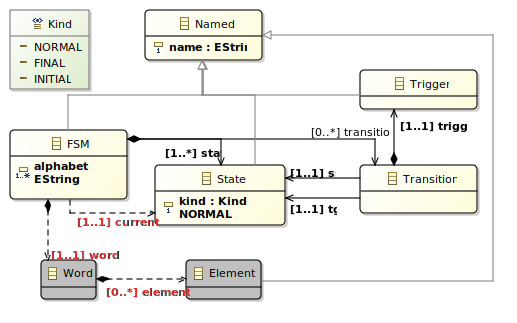
\includegraphics[width=\columnwidth]{FSM}%
   \caption{A metamodel for Place/Transition Petri Nets.}%
   \label{fig:FSM_MM}%
\end{figure}



\subsubsection{Execution}
\label{sec:Examples:PN:Execution}

Starting with an initial marking, i.e. setting the values of \textsf{marking} for
each \textsf{Place} appearing in a model, executing a \textsf{PN} consists in 
sequentially \emph{firing} enabled \textsf{Transition}s, until no 
\textsf{Transition}s are enabled any more. A \textsf{Transition} \textsf{t} is 
\emph{enabled} iff each input \textsf{Place} (i.e. a \textsf{Place} connected to
\textsf{t} by an \textsf{Arc} directed to \textsf{t}) is marked with at least the
weight of the \textsf{Arc}. Firing \textsf{t} consumes tokens from all input 
\textsf{Place}s and creates tokens on output \textsf{Place}s, according to the
corresponding \textsf{Arc}s' \textsf{weight}. Not that an enabled \textsf{Transition}
may not fire, denoting concurrency and non-determinism.

\subsubsection{Animations}
\label{sec:Examples:PN:Animations}

Typically, the execution semantics is implemented with a transformation unit 
\textsf{step} that would select one enabled \textsf{Transition} among all possible,
and \textsf{fire} it. The execution stops when no \textsf{Transition}s are enabled
any more. There is several possibilities for animation.

\begin{description}
   \item[PN.1] Highlight all \textsf{Transition}s that are enabled;
   \item[PN.2] Highlight \emph{the} \textsf{Transition}, among all enabled ones,
   that has been selected for firing;
   \item[PN.3] Firing a \textsf{Transition}, which may be realised using 
   different animations:
   \begin{description}
      \item[PN.3.1] Removing, at once, all markings from input \textsf{Place}s 
      and creating new, additional markings on the output \textsf{Place}s.
      \item[PN.3.2] Removing/Creating the markings, but sequentially on all input
      \textsf{Place}s.
      \item[PN.3.2] Removing/Creating the markings as before, but ``sliding'' the
      tokens along the \textsf{Arc}s to visually represent the marking transfer.
   \end{description}
\end{description}
Again, all those three animations are related in complex ways: it may be possible
to perform them step by step, or automatically, or even interactively leave the 
choice to the user to select which \textsf{Transition} has to be fired. 